\documentclass{report}
\usepackage[
top    = 2.75cm,
bottom = 2.50cm,
left   = 3.00cm,
right  = 2.50cm]{geometry}
\usepackage{hyperref}
\usepackage{cite}
\usepackage{setspace}
\usepackage{algorithm}
\usepackage{algpseudocode}
\usepackage{graphicx}
\graphicspath{ {./images/} }
\title{\vspace{-2.0cm} A Generalizable Framework for Automated Cloud Configuration Selection \\ \vspace{0.5cm} \large Supervisors: Adam Barker \& Yuhui Lin}
\date{2019-06-06}
\author{Jack Briggs - 140011358 \\ MSc Data-Intensive Analysis}
\doublespacing
\begin{document}
\pagenumbering{roman}
\maketitle
\newpage
\chapter*{Abstract}
Outline of the project using at most 250 words
\newpage
\chapter*{Declaration}
I declare that the material submitted for assessment
is my own work except where credit is explicitly
given to others by citation or acknowledgement. This
work was performed during the current academic year
except where otherwise stated.
The main text of this project report is NN,NNN* words
long, including project specification and plan.
In submitting this project report to the University of St
Andrews, I give permission for it to be made
available for use in accordance with the regulations of the University Library. I also give permission for the title and abstract to be published and for copies of the report to be made and supplied at cost to any bona fide library or research worker, and to be made available on the World Wide Web. I retain the copyright in this work.
\newpage
\tableofcontents
\listoffigures
\newpage
\pagenumbering{arabic}
\chapter{Introduction}
\section{Cloud Computing}
Cloud computing is an ever-growing field that now ranges from Infrastructure-as-a-service (IaaS) to Software-as-a-service(SaaS). Services under cloud computing are characterised by their ability to offer access to a shared pool of highly elastic on-demand computing resources that offer broad network access \cite{Pallis2010, Mell2011}. Cloud services as an industry has had an explosive growth, and it has been predicted that 83\% of enterprise (Companies with 1000+ employees) workloads will be in the cloud by 2020\cite{Intricately2019}, with 41\% run on public cloud platforms such as Amazon AWS and Microsoft Azure. Services offered range from various levels and forms of abstractions, from directly provisioning Virtual Machines (VMs) or storage services, allowing users full control over their cloud infrastructure, to deploying 'serverless' containers, where the actual managing of the hardware is instead handled by the cloud provider.

\paragraph{}
The appeal is obvious, with cloud services allowing organizations and developers to utilize a diverse range of computational resources on demand without any up-front commitment or cost \cite{Armbrust2009}. This can lead to both significant cost-savings as well as improved revenue through better customer experiences and enabling risk-free experimentation\cite{Power2018}. Academics, too, are utilizing the available services as volumes of data grow impractical to store and analyse on local machines\cite{Berriman2013, Ruiz-Alvarez2011}. This includes large-scale collaborative projects involving huge data sets hosted on the cloud such as the 1000 Genomes Project\footnote{\url{https://aws.amazon.com/1000genomes}} or Common Crawl\footnote{\url{commoncrawl.org}}.

\subsection{Cloud optimization}
A wide range of applications are now deployed on cloud machines or make use of objects stored on them, from large-scale data analytics jobs mentioned to media-streaming servers such as Netflix or Twitch\cite{Bilal2017}. The resource dependencies of these applications similarly vary widely, from the CPU dependent data analysis tasks to network-heavy streaming services. Virtual machines offered by different cloud providers vary in terms of memory amounts of number and speed of virtual CPUs (vCPUs), and each application's performance will have different relationships with these options. While medium-length video transcoding operations will benefit primarily from faster processing speeds, data analysis tasks involving large datasets may find a more cost-effective option in prioritising VMs with a local solid-state drive (SSD) offering high I/O performance. Non-critical batch workloads can often benefit from using 'pre-emptible' or 'spot' instances, which offer large discounts on the condition that your machine can be terminated with little notice to free up resources. 

\subsection{Benefits}
It is desirable for both users and providers to maximise the optimize purchased cloud configurations to best serve the needs of their applications. Users or developers who fail to do this risk paying far more than they need to for the same performance. A given data analysis task can cost around 3.4 times as much on an average configuration compared to the optimal available option\cite{Alipourfard2017}. Even serverless frameworks simply shift the burden of optimization from the users to the cloud providers. For cloud providers too, efficient deployment across available Virtual Machines frees up extra resources available for other purposes or other customers. Alternatively, identifying and avoiding the co-location of CPU intensive workloads can reduce resource contention amongst users, leading to improved performance \cite{Pu2010}. In addition, energy-related costs make up to 42\% of managing a data-centre, and the ability to idle inactive resources would lead to a significant reduction both in energy cost and environmental impacts. \cite{Berl2010, Gkatzikis2013}. 
% It'd be nice to show some hard numbers to show the benefit of optimizations, like the market share or something, but obvoiusly that's pretty hard
% Cloudability?

\subsection{Challenges}
Picking an optimal cloud configuration for any given application is far from trivial. 'Larger' VM types may not provide improved performance \cite{Yadwadkar2017}, or may do so at a far less cost-efficient rate. Even if one knows their exact budget along with the constraints placed on their application's performance, they must still find a way to search or model across the entire range of cloud providers to ensure they have found the optimal cloud configuration for their application. This is further complicated by the variety of instance types available across multiple providers, and the variation in performance between virtual machines of the same specification due to differences in underlying hardware, network traffic, and co-located tenants located on the same physical machine.

\subsubsection{Search space}
The diversity in services provided by different cloud providers creates a large search space. At the time of writing, Amazon EC2\footnote{\url{https://aws.amazon.com/ec2/}} alone offers over 200 predefined instance models\footnote{\url{https://www.ec2instances.info}}, while Google Compute Engine\footnote{\url{https://cloud.google.com/compute/}} allows users to define their own machine types, ranging from small VMs with 1 vCPU and 1 GB of RAM to 96 vCPUs with 624 GB of RAM\footnote{\url{https://cloud.google.com/custom-machine-types/}}, and includes options for specifying the CPU platform or adding GPUs. VMs can also differ in terms of network performance, local storage, and CPU speed, underlying hardware, and can start able to run a variety of operating systems and associated software. 
\paragraph{}
The search space is not just challenger in terms of range, but is also hard to define in terms of constraints. Many hardware options are precluded by or only permitted alongside other options. To simplify selection, leading providers generally categorize instance types are generally split into categories such as 'compute-optimized' and 'memory-optimized' machines, each of which is made up of machines of various 'sizes,' such as 'tiny,' 'small,' 'large,' referring to the computational resources available to that virtual machine. Even with this categorization, it can be hard to formalize or encode the search space in such a way to best serve an automated optimization software.
\subsubsection{Hardware and Software Heterogeneity}
Despite two Virtual Machines sharing the exact same configuration, if their underlying machines possess different physical hardware then their performance can differ significantly\cite{Leitner2014}. Amazon's M4 instance types, for example, can come with either 2.3 GHz Intel Xeon® E5-2686 v4 (Broadwell) or a 2.4 GHz Intel Xeon® E5-2676 v3 (Haswell), based on the machine they happen to be hosted by\footnote{\url{https://aws.amazon.com/ec2/instance-types/}}. However, more recent studies involving newer instance types have shown a dramatic reduction in this CPU-based variability for certain instance types\cite{Davatz2017, Laaber2019}. 
\paragraph{}
Problems regarding hardware heterogeneity expand further when searching across multiple providers. Different providers may use vary different hardware for machines reporting the same number of vCPUs or disk speeds. Software too, can differ. Amazon instances come configured according to a template referred to as an Amazon Machine Image (AMI)\footnote{\url{https://docs.aws.amazon.com/AWSEC2/latest/UserGuide/AMIs.html}}, while Google Compute Engine instances use a predefined boot disk. These images include an operating system and associated software, storage snapshots, launch permissions, and device mappings. The APIs used to communicate with cloud providers in order to set up cloud services in the first place similarly differ between providers. Even when using Infrastructure as code (IaC) tools, the nomenclature and configuration file structure can differ widely.
\paragraph{}
When searching across multiple instance types, the hardware and software heterogeneity must be taken into account, especially when the search spans separate cloud providers. 
\subsubsection{Variation}
Even when run on identical cloud configurations from the same provider, the same application or benchmark can have significantly different performance, more so than is observed when run in on-premise environments\cite{Leitner2014}. This is in part due to the hardware heterogeneity in underlying machines described above, but can also occur due to multitenancy. Multiple customers may share computational resources by running VMs on the same physical machine. This can lead to a slowdown in one instance due to the behaviour of another colocated tenant. This problem is referred to as the 'noisy neighbour' problem\cite{Gkatzikis2013}. Disk I/O operations or network traffic between instances and storage disks could similarly be affected by the machine's relative locations within or between datacentres. 
\paragraph{}
All the above problems causing variation within instance types are generally out of the control of the customer. Cloud providers may be develop methods of minimising the problems, shown by the reduction in the variation of intra-cloud network performance\cite{Scheuner2018a} and CPU performance between identical instance types \cite{Davatz2017, Laaber2019}.  Nonetheless, in cloud configurations where this variation is still significant, it add a significant element of randomness to the performance of various applications on cloud services. This randomness must be accounted for by any method used to optimize cloud configurations, and rules out assumptions of deterministic application performance. 
\subsubsection{Application range}
As mentioned earlier, numerous types of applications are deployed on the cloud, from long-running web-servers and media-streaming services to one-time data analytics jobs. The performance and cost-effectiveness of these applications can have very different non-linear relationships with cloud configurations, making them difficult to model analytically, even if the contents of the application are known exactly. In some cases, such as in serverless container services such as Google Cloud Run\footnote{\url{https://cloud.google.com/run/}} the application is not known at all, and must be treated as a black box. \\
To ensure an optimization method is as generalizable as possible, it must be able to utilize user's specifications and the outputs of an application, but must treat the application itself as a black box, and not make hard assumptions regarding any of its characteristics or relationships with configuration options.
\subsubsection{Objective measure}
Finally, the very meaning of the word optimal can depend on the application and the user. The ultimate goal is far from fixed, as optimizing for a good mean performance for a server may fail to optimize for high stress situations, leading to lower-than expected performance under these conditions. Even in single batch jobs, different users may tolerate different reductions in performance for different cost-savings. While an effective option is to simply present to the user an informative representation of how cost and performance vary with cloud configuration options, this is not possible in many black-box options, and limits the degree of automation in the optimization process.\\
To truly automate an optimization process for any provided application, an 'objective measure' must be provided, dependent on cost and performance, which reflects the ultimate goal of the optimization process. An optimization method must be able to accommodate different user requirements through flexibility regarding the objective measure used.

\section{Aims and Objectives}
% Also say that you'll use the results to see how different search options are affected/variability, whatevs
The aim of this project is both to present a framework for completely automated selection of an optimal cloud configuration for any given application, as well as to deliver a fully functional implementation of this framework for an indicative use-case. To achieve this aim, the framework must achieve the following objectives:
\begin{itemize}
\item Present a fully automated process for optimization cloud configuration.
\item Be applicable for any form of cloud application.
\item Not be limited to any one cloud provider or service.
\item Take into account variation within and between instance types.
\end{itemize}
The framework should require only the following inputs, from which it should output a single estimate for the optimal cloud configuration:
\begin{itemize}
\item The application itself, to be set up on a given cloud service.
\item Details of the search space and its constraints.
\item An objective measure with with to evaluate cloud configurations.
\end{itemize}
In addition, we wish to deliver a fully functional implementation for an indicative use case, which will achieve the following objectives:
\begin{itemize}
\item Automate selection of cloud configuration samples based on a search space of cloud configurations spanning multiple providers.
\item Provision specified instance types from multiple providers based on a given cloud configuration.
\item Deploy and return logs for a given application on a given cloud service based on a given cloud configuration.
\item Interpret logs based on the performance and cost of a given application on a given cloud configuration.
\end{itemize}
\section{Contributions}
% Do after evaluation
\section{Dissertation Outline}
% Structure
\chapter{Literature Survey}
\section{Cloud services}
% Evidence of the cloud market growing
% Examples of its use, and how optimization is used
% Types of cloud offers that now exist (Kubernetes clusters, serverless, etc.)
\section{Cloud variability}
% How variability of the cloud has been reported
\section{Optimization methods}
% Previous optimization methods that have been attempted
% Modelling vs Benchmarking vs Searching
%http://www.brendangregg.com/blog/2017-12-31/reinvent-netflix-ec2-tuning.html
\subsection{CherryPick}
\subsection{PARIS}
\subsection{Ernest}
\subsection{Daleel}
\subsection{Okta}
\subsection{OTHERS, LOOK UP}
asdf
\subsection{Exhaustive search}

% Not exactly an actual type, but the obvious alternative.
\section{Benchmarks}
% When using benchmarks, some choice as to which one to use. What makes a good benchmark.
\subsection{Cloudsuite}
\subsection{vBench}
\subsection{OTHERS, LOOK UP}
\section{Infrastructure-as-code}
\subsection{Terraform}
\subsection{Apache Libcloud}  
\subsection{Chef}
\subsection{Puppet}
\chapter{Requirements specification}
\section{Use-case}
\subsection{Bayesian Optimization}
\subsection{Video transcoding}
\section{Requirements}
% Accommodating flexibility with how confident the program must be
% Reduced predictive power may be acceptable for substantially reduced search cost/time, depending on the user 
\section{Optional Requirements}
\chapter{Generic Automated Cloud Configuration Optimization Framework}
% Architecture shows predifined subroutines for each component, we go into details of what these entail in their respective sections
% START HERE
\section{Design Motivations}
\subsection{Numerical Optimization}
In any optimisation process, the value of some objective function is minimised or maximised by adjusting its input variables or parameters. An optimisation algorithm begin with an initial guess of these variables and iterates through improved estimates until they terminate, hopefully providing an estimated solution \cite{Nocedal2006}. An optimization function effectively takes previous an objective function, along with its previous inputs and outputs as arguments, and outputs either the next sample to take, or the predicted best input if the stopping condition is met. \\
In our generalized case, the optimisation method and objective function are both unknown, but we know that our objective function will always involve selecting some cloud configuration based on the inputs that describe that configuration, deploying some application onto this configuration, and interpreting its performance to give some objective measure.
 

\subsection{Modularity}
In our generalized case, we do not yet know the optimization method or objective function. As shown in our Literature review, a number of optimization algorithms have been attempted and are available, such as exhaustive search, Bayesian optimization\cite{Alipourfard2017}, analytical methods that directly model the application's relationships with configuration variables\cite{Venkataraman2016}, and a data-driven approach predicting performance by its relationship with pre-run benchmarks\cite{Yadwadkar2017}.

Much like how our objective measure will differ from application to application, the best optimization method may also differ depending on the type of application tested. Applications whose performance is accurately reflected by known benchmarks may benefit from PARIS's data-driven approach, while situations with unclear non-linear relationships to configuration variables will be well suited to Bayesian optimization. Because of this, while we will focus on developing an implementation of Bayesian optimization, as per our use case, it is desirable to ensure that our example optimization method can be replaced by another if the user deems it more appropriate to their use-case.

Because of this, we are left with multiple parts of our system which are highly dependent on a user's individual use-case, namely the objective function, the objective measure to be optimized, the search space constraints, and the application itself. Because of this, we have taken a highly modular approach to our design. While our implementation should be self-sufficient to run its example case, it should also be made up of several replaceable components for future extensions. The framework itself should be well suited to any case, while each individual component, the user can pick the specific implementation that is best suited for their use-case.
 
\section{System Architecture}
\begin{figure}[!hb]
  \centering
   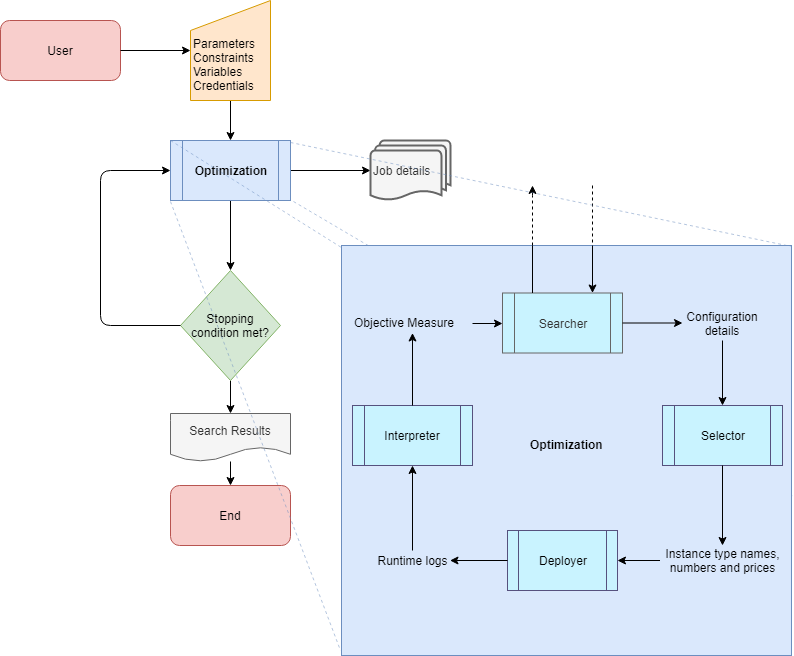
\includegraphics[scale=0.5]{Design_flowchart}
  \caption{A flowchart showing the processes involved in and information flow through the designed system.}
  \label{fig:design}
\end{figure}
\newpage
Our optimization process can be broken down into four replaceable components: A Searcher, which runs the optimisation algorithm, testing out various inputs in an attempt to maximise or minimise the objective function; a Selector, which interprets the inputs to determine what cloud configuration is being tested; a Deployer, which provisions the machines needed for that cloud configuration, deploys the application, and once it has terminated returns any required logs from it; and an Interpreter, which takes these logs to calculate the objective measure which is returned to the Searcher as the returned value for the objective function. A diagram of this breakdown is shown in figure \ref{fig:design}. The components themselves are examined in further detail in the following sections.
 
\paragraph{}
Overall, the system drives forward an optimization algorithm shown in Algorithm \ref{alg:Optimization}, such as Bayesian optimization, coordinate descent, random search, or exhaustive search, by iterating through potential input variables. For each set of these inputs, it take a sample from a single 'job,' where it runs through a single loop of the Selector, Deployer, and Interpreter components. The Searcher component then uses the results from inputs tried so far to choose the next set of input variables to sample, as well as provide the current estimate of the best possible set of input variables to minimize or maximize that result. Once the stopping conditions are met, the latest estimate for the best input variables is output by the system.

\begin{algorithm}
\caption{Optimization Procedure}
\label{alg:Optimization}
\begin{algorithmic}
\Procedure{Optimization}{$Starting \ variables, Stopping \ conditions, Searcher, Selector, \newline
\hspace*{4.3cm} Deployer, Interpreter$}
\State $\vec{x}_{0}\gets Starting \ variables$
\For{$i = 0,1,2,3,...$}
\State $Config_i, Price_i\gets Selector(x_i)$
\State $logs_i \gets Deployer(x_i, Config_i)$
\State $results_i \gets Interpreter(x_i, logs_i, Price_i)$
\State $\vec{x}_{i+1}, stop, best\vec{x} \gets Searcher((x_-, x_1,...x_i), (results_0, results_1,...results_i),\newline
\hspace*{5.6cm}Stopping\ conditions)$
\If{$stop$} 
\State \Return $best\vec{x}$
\EndIf
\EndFor
\EndProcedure
\end{algorithmic}
\end{algorithm}
 

\paragraph{}
It is assumed that in the vast majority of cases, the user would provide their own Interpreter and Selector. Interpreters and Selectors are very dependent on the form these logs will take, and the form the search space will take, and are extremely hard to generalise. For this reason, the modular design of our solution should make it simple for any component to be supplied or replaced by the user.  \\
While Interpreters and Selectors are highly specific, in only some cases should the user need to provide their own Deployer. Applications can often be contained within Docker containers, complete with requirements and runtime instructions. Because of this, aside from occasional setup, for example in multi-node clusters or multi-container applications, a Deployer which provisions a given configuration from a given provider, and then deploys and attaches to a user-provided docker image to collect its logs will be sufficient.  \\
Only in rare cases would the user be required to provide their own Searcher. This is because optimization algorithms themselves should be applicable to any deployment. While, as mentioned, in some cases different searchers may be more effective, Bayesian Optimization is a good general method for predicting an application's optimal cloud configuration with reasonable accuracy with very few samples. A Bayesian Optimization implementation will be provided.


\section{Inputs and outputs}
The user inputs are shown in figure \ref{fig:design} as being made up of 4 parts: Parameters, constraints, variables, and credentials. The parameters would be options for the searching method itself, such as the stopping conditions or maximum number of concurrent jobs. Variables and constraints together define the possible search space for the input variables, as well as their starting values. Each variable must be given a type, such as string or integer, and a set of constraints such as maximum or minimum for numeric variables or the available options for categorical variables such as strings. Finally, the user would have to submit paths to the files holding the credentials to allow the program to provision and access virtual machines on the tested cloud providers. It is of course essential that credentials are never stored in any form by the program itself, and only paths to the relevant files are passed to the relevant tools and interfaces.
\paragraph{}
The figure also shows the relevant outputs created by the system, in the form of 'job details' and 'search results' output as files containing details describing the jobs performed and their individual results, as well as the final prediction for the optimal configuration produced by the system. Keeping outputs from individual jobs is important, both for debugging the system during development or component switch-over, as well as to allow users to avoid repeating unnecessary repeats of already tested configurations when performing multiple search experiments.
\paragraph{}
Algorithm \ref{alg:Optimization} shows the general form the optimization process takes with only one concurrent job allowed at any time, showing the expected input and output of each individual component. These are explained in more detail within each component's individual section below.

\section{Searcher}
The Searcher component is actually responsible for handling the optimization algorithm itself. The Searcher takes the results from previous jobs and determines either the next best sample to take within the available search space, or to terminate the process and return the current best prediction for the optimal configuration. 

\paragraph{}
A perfect Searcher is one that returns a perfect prediction of the optimal configuration in as few samples as possible. Fewer samples means a reduction in the time and cost taken to perform the search. Often, there is a trade-off here, where extending a search to include more and more samples, such as by setting less restrictive stopping conditions, increases its predictive accuracy.

\paragraph{}
As an example, in an exhaustive search every possible combination of the inputs is sampled, giving a complete analysis of the entire search space. This obviously takes many samples, $n * \prod_{i=1}^{j} x_{i}$ where $x_{i}$ is the number of options for the \textit{i}th of J variables, and n is the number of samples taken from each configuration. This results in a large or even infinite search cost and time, but is almost certain to return the optimal result, depending on the amount of randomness involved in sampling.

\paragraph{}
Unless a job is repeated on an extremely regular basis, a user will likely desire to give up a small degree of accuracy or generalizability for a dramatically reduced search cost or search time. Some search methods, such as PARIS\cite{Yadwadkar2017}, can leverage past search experiments to reduce the number of samples taken. Generally however, the stopping conditions and search method will control this trade-off, and can be set according to the user's search budget or time constraints. 

\paragraph{}
In order to accurately predict the best next sample to take, the Searcher must know the available search space.  A description of how to encode cloud configurations into a set of variables and constraints is done in the Selector section. Ideally, we want our searcher to be capable of performing multiple jobs concurrently.

\section{Selector}
The Selector interprets the variables provided by the Searcher component into the form of an available cloud configuration. Cloud configurations have a number of variables that can describe them, such as vCPU number, memory amount, disk speed, number of instances, instance category, machine type, and cloud provider. The selector must use whatever combination of these is provided and find either the exact or most similar cloud configuration available, passing this information on to the Deployer. In the tools used for our implementation, no cross-provider API was available to directly translate machine specifications into the virtual machine types available from different providers.

\subsection{Exact vs. Closest Match}
For finding an exact match, the Selector can simply lookup the appropriate instance type from a dataset according to the input variables stored as each instance type's attributes. Looking for a closest match rather than an exact one gives more flexibility in how the input variables can be encoded, but means more complicated decisions such as attribute priority must be made, and extra assurances made to not repeat unnecessary samples when multiple sets of inputs describe the same closest input type. For our use-case, we will specifically use the simpler Exact Match method, but thanks to the modular design it will be easy to extend to include a Closest Match Selector option if time allows.


\section{Deployer}
The Deployer deploys the user-provided application, batch job, or benchmark onto the selected cloud configuration, and collect any necessary analysis from it. Typically this will involve provisioning the necessary machines from the given provider, followed by deploying the given application onto these machines, and either collecting logs from them or from a networked instance or cluster. 

\subsection{VM Provision}
Aside from in serverless computing, a necessary step of deploying any cloud-based application is provisioning the virtual machines themselves from a cloud provider. The Deployer should be capable of requesting any virtual machine chosen by the Selector, regardless of provider. This can be simplified using Infrastructure as code (IaC) tools such as Terraform, which offers the ability to codify the APIs from many different providers into declarative configuration files. As long as configuration files and credentials for use by an IaC tool are supplied for each possible provider, then a Deployer can call the corresponding IaC tool to provision the machines. 
There are several requirements for the IaC tool that is used. As instance type and number of machines will be supplied by the Selector, and therefore cannot be known until the machines are provisioned, either they must be declarable as variables when the tool is run, or the configuration files must be suitable for automated editing just beforehand. Along with this, the tool must support multiple concurrent tasks with their own specifications and outputs, if we hope to allow the Searcher to take multiple samples at once.

\subsection{Application Deployment}
Once the Virtual Machines themselves are provisioned, the application must be set up on them and run. There are many forms this application can take. For our use-case, we have assumed the application is fully contained within a single Docker image. This enables effective deployment both on single machines as well as by cluster-based container-orchestration systems such as Kubernetes. Pre-built Kubernetes clusters are offered by several leading cloud providers. However, other types of applications are common, such as micro-service based web applications. Alternatively, an application's performance might be best estimated by its response over a network, and poorly estimated internally. Once again, the modular design allows users to implement their own Deployers to deal with alternative situations. 

\subsection{Simulated Deployment}
It may be advantageous, especially during debugging or if using a 'closest match' approach to configuration selection, to instead either simulate the response from provisioning and deployment of an application, or to return a previously sampled response. To this end, it may be useful to ensure full logs of any deployment are stored so that, if desired, future calls to 'Deploy' an already sampled configuration for a given application can simply be responded with a randomly distributed value based on previous results from the same configuration.

\section{Interpreter}
The Interpreter must interpret whatever logs and other information is returned by the Deployer, along with the cost of the cloud configuration provided by the Selector, in order to return an objective measure for the sampled cloud configuration. It is this returned value that the Searcher will be attempting to minimise or maximize. We leave it to the user to develop an Interpreter for their use-case. This will likely involve extracting relevant information from the deployed application's logs, and applying constraints based on the time taken or machine pricing. 

\chapter{Bayesian VM Optimization System}
In this chapter we describe the design considerations for the example use-case implementation we provide for our framework.

\section{Bayesian Optimization}
Bayesian Optimization is an optimization method specifically designed for situations where the objective functions itself is unknown beforehand and expensive to perform, but can have its outputs directly observed through experiments\cite{Snoek2012}. It models the objective function as a stochastic process, a 'prior function,' and computes its confidence intervals based on samples. Using these confidence intervals and a pre-defined acquisition function it decides future samples to take based on where there it estimates there to be the most potential gain. A diagram showing this process is shown in figure \ref{fig:cherrypic}. By this process Bayesian Optimization can find optimal or near-optimal solutions for any non-parametric problem in a relatively small number of samples compared to other optimization methods. In addition, whereas other methods, such as exhaustive search, may handle uncertainty through sampling results from the same inputs multiple times, Bayesian Optimization can incorporate this uncertainty into its estimates, further reducing the number of samples needed.

\begin{figure}[!hb]
  \centering
   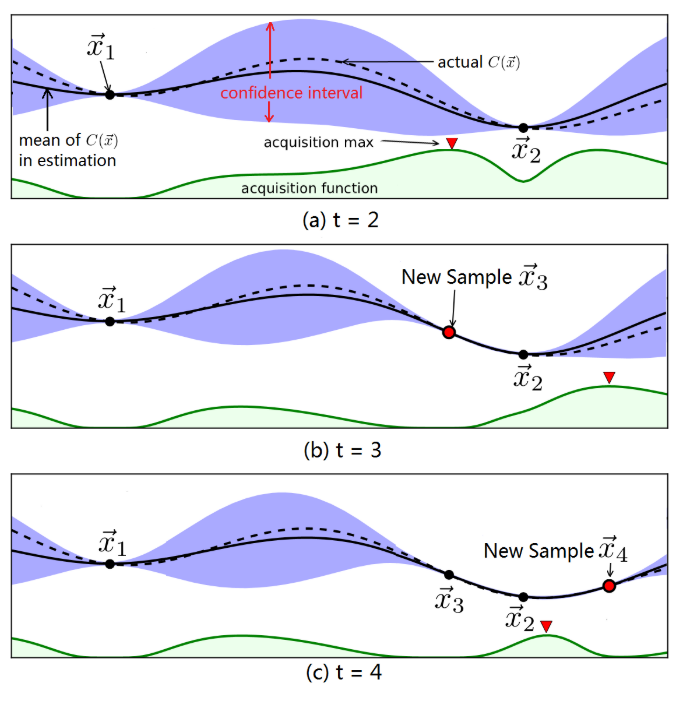
\includegraphics[scale=0.5]{Cherrypic}
  \caption{An example of BO's working process. Taken from Figure 5 in \cite{Alipourfard2017}}
  \label{fig:cherrypic}
\end{figure}

There are a number of possible prior functions, acquisition functions, and stopping conditions that can be used with BO, and the Cherrypick paper goes into detail on the reasoning behind which options are best for cloud configuration selection specifically\cite{Alipourfard2017}. Some notable differences in our case, however, is that CherryPick was specifically focused on batch jobs, where what is measured is simply a function of an instance type's cost and its time taken to perform a given job. Its acquisition function is specified to this purpose, minimizing costs but biased towards configurations which satisfy a soft performance constraint by successfully performing the batch job within a given time. In our case, our acquisition function must be more general, and we will therefore be relying on the user to ensure that whatever objective measure it returned by their Interpreter has already taken into account soft or hard performance constraints such as this.
\section{VM Docker Deployment}
Once the VM itself has been provisioned, the application must be deployed onto them. In the use case, we assume that the application being tested is available in the form of a Docker image, and that a single instance is provisioned on which to run that application. Docker offers a remote API with which to direct the host machine to download an image and run a container based on it, as well as returning an application's logs. In order to deploy an application onto a VM, that instance must first have Docker installed onto it and Docker directed to a public-facing port. The Deployer can then use the public facing IP of the provisioned machine along with user-provided security credentials to deploy the application. The Deployer can then obtain and return any and all logs the deployment produces for use by the interpreter.

\section{Search space encoding}
Whether using exact or closest match, it must be decided how to encode cloud configurations into a set of input variables. This problem is further complicated by the fact that constraints for certain inputs may depend on the values of others, as is often the case in cloud computing. Large memory amounts are often only available on machines with more vCPUs, and some providers may offer available configurations others do not. Google Cloud Platform allows users to specify custom machine types, but even these do not allow any possible combination (for example, Memory constraints are tied to vCPU number, and vCPU number must be divisible by 2).

\paragraph{}
Despite these problems, there at at least clear patterns prevailing throughout leading cloud providers, such as separating machine types into categories equivalent to 'Compute-optimised', 'Memory-optimised', and 'Storage-optimized,' each with a set of machines with between 2 and 96 CPUs. In lieu of a cross-provider service to match a given specification to a specific cloud instance type, something which would be outside the scope of this project, these industry-standard categorisations can be used to encode the search space in a reasonable manner. Table \ref{tab:config-encode} shows an example of how we have used these patterns to encode 6 instance types into a set of 3 easily interpreted variables; Provider, vCPU number, memory, and machine category. A searcher tool could easily filter a dataset of this form to find the instance-type for a set of input variables.

\begin{table}[!t]
\centering
\begin{tabular}{ |c||c|c|c|c|  }
 \hline
 Instance Type & Provider & Category & vCPU Number & Memory \\
 \hline
 n1-standard-2    & GCE  & General & 2 & 7.50 \\
 n1-standard-4    & GCE  & General & 4 & 15.00 \\
 n1-standard-8    & GCE  & General & 8 & 30.00 \\
 c5.large         & EC2  & CPU & 2 & 4.00 \\
 c5.xlarge    & EC2  & CPU & 4 & 8.00 \\
 c5.2xlarge    & EC2  & CPU & 8 & 16.00 \\
 \hline
\end{tabular}
\caption{A possible way of separating instance types into 4 descriptive variables. Providers were either the Google Compute Engine (GCE) or the Amazon Elastic Compute Cloud (EC2)}
\label{tab:config-encode}
\end{table}

In the end,  however, the important features and constraints for the search space will differ for each user, and it may be beneficial to run multiple experiments in different search spaces before settling on a final decision for an instance type. While we provide in our associated implementation an example of how to encode and select available cloud configurations for our Bayesian Optimization tool, we think it best to ultimately leave it to the user to design and implement a Selector system that works well for their specific use-case.
\section{Objective Measure}
Our video transcoding benchmark returns the time taken to transcode a given video file, relative to a reference. We have assumed that our ultimate goal is to find the cloud configuration that will maximise the amount of video transcoding performed per unit cost.  In a competitive business environment, even a small increase in transcoding speed may translate to large increases in customer uptake, but our simple metric should effectively show how an benchmark score can be used with an instance price to generate an objective measure.

The vBench benchmark used, 'vod', returns a 0 if the video quality is not of a sufficient quality following transcoding. This effectively sets a hard constraint on performance, ensuring that no matter how cheap an instance is, it must achieve a certain level of performance to be selected.
Cherrypick\cite{Alipourfard2017} instead incorporates constraints into the Bayesian Optimziation algorithm itself by including it within the acquisition function. This is not an easily generalized solution, and so it not replicable in our case. We have instead incorporated performance constraints within the objective measurement itself.

\chapter{Implementation}
\section{General usage}
Our solution was implemented with a combination of Bash scripts and Python 3. Exhaustive search was performed using simple Bash scripts. The Searcher component was implemented using Spearmint\cite{Snoek2012}, an implementation of Bayesian Optimization in Python. Due to the design of Spearmint, the Searcher component was made to call a single core python script that would call user-specified functions that make up the Selector, Deployer, and Interpreter components. Several components were implemented, each in the form of separate Python functions. Extension of the solution by adding additional components is easily done by writing new Python functions that either directly perform the component's job or calls another tool to do so.

User-provided options, such as what Selector, Deployer, and Interpreter to use, as well as other user supplied variables can be provided in the form of a JSON file that is read and loaded as a Python dictionary by this core script. This dictionary is passed as input to each component, which are able to update it with any information needed by other components in the form of key-value pairs. At the end of any job, this dictionary object is saved in JSON format for later analysis and recovery of previous results.

\section{Searcher}
\subsection{Spearmint}
Spearmint is an implementation of Bayesian Optimization written in Python. The user submits a single python script with an appropriate 'main' function which has its inputs optimized. It provides numerous settings for changing variables like the maximum number of concurrent jobs, acquisition function, and sampling noise assumptions. However, the latest available implementation of Spearmint was found to be outdated and incompatible with the latest versions of various Python modules used in later steps. 
Because of this, for the sake of generalisability we first updated Spearmint to be compatible with Python 3 and newer versions of its dependencies such as Google Protocol Buffers. This implementation of spearmint has been made available\footnote{https://github.com/briggsby/spearmint3}. The edits mostly included changes to syntax inconsistent with new versions of its dependencies.

\subsection{Search space encoding}
Spearmint uses their own protocol buffers to allow users to specify the available input variables. Each variable must be typed as either an integer (INT), floating-point number (FLOAT), or categorical variable (ENUM). For the first two, minimum and maximum limits must be set, while for categorical variables each available option must be specified. For all variables, a 'size' is specified, and each variable is passed to the function as a Numpy\cite{Klein2014} array with a number of elements equal to its 'size.' Each of these elements is optimized individually.

This format of encoding variables sets some limitations. Constraints for numeric values are limited to minimum or maximums. For example, vCPU number for custom instance types on Google Compute Engine are limited to even numbers. While there are methods to get around this, such as encoding vCPU number as an integer which is then multiplied by 2 by the submitted script, it can lead to repeated job failures as impossible inputs are repeatedly attempted.

To get around this problem, the vCPU number was specified instead as a categorical variable, and other than that the encoding is identical to that described in the Design section:
\begin{enumerate}
\item vCPU number was encoded as a categorical variable of size 1 with options '2', '4', and '8.' 
\item Provider was encoded as a categorical variable of size 1 with options 'aws' and 'google', corresponding to Amazon EC2 and Google Compute Engine respectively.
\item Category was encoded as a categorical variable of size 1 with options 'General,' 'Memory,' and 'CPU.'
\end{enumerate}
\section{Driver}
The Driver script is a single python file called by Spearmint, and as such must take as parameters only the Job ID (a number used to identify jobs within a single spearmint experiment) and input variables as a multidimensional array.\\
The Driver immediately reads a local configuration file in JSON format and loads it as a Python dictionary. This configuration dictionary stored relevant information in a set of key-value pairs, such as the user-specified Selector, Deployment, and Interpreter components, and other variables such as the Docker image address and container runtime commands. The key and value are specified within the files to make sure the system is extensible to any later added components. This configuration dictionary is updated with the input variables submitted with that job, is passed as a parameter to the functions specified as the framework components, and is saved to a local JSON file at the end of the job for record-keeping and debugging purposes. \\
The driver file responds with a single value, the objective measure to be minimized by the Bayesian Optimization process.
\section{Selector}
\subsection{Exact Match}
A CSV file was created with the following variables for the instance types used in our evaluation:

\begin{itemize}
\item API Name - Name of instance type used in that provider's APIs (string)
\item Provider - Cloud provider offering the instance type (string)
\item CPU - Number of vCPUs (float)
\item Memory - Amount of memory in GB (float)
\item Category - Category of machine type, such as Compute or Memory optimized, in a consistent form between providers (string) 	
\item Price - Hourly cost of the machine for an On-demand Linux image (float)
\end{itemize}

The selector loads this dataset as a Pandas dataframe, and filters it according to the input variables provided. The configuration dictionary is then updated with the API name and hourly cost for the cheapest option remaining, and returned by the function. If not configuration is left in the filtered dataframe, these values are instead set to a Null value, to indicate that no configuration exists.

\section{Deployer}
\subsection{VM Provisioner}
The first stage of any tested deployment was to first provision the necessary virtual machines from their cloud provider. To do this, we implemented the Infrastructure-as-code tool Terraform, using a Python library python-terraform\footnote{https://github.com/beelit94/python-terraform}. 
\subsubsection{Terraform}
Terraform operates by applying 'plans' based on Terraform configuration files and variables provided either during the applying step or in separate 'tfvars' files. For each provider, a separate folder was created with a corresponding Terraform configuration file. The configuration files would, when applied using Terraform, provision a number of machines of a given type, and set up a publicly accessible Docker host on each machine. This is done by first setting up a security rule exposing a specific port later used by Docker. The machine of the given type is provisioned, and using SSH Docker is installed, using either the Amazon Linux Extra library\footnote{\url{https://docs.aws.amazon.com/AWSEC2/latest/UserGuide/amazon-linux-ami-basics.html\#extras-library}} for AWS machines, or using a downloaded script from \url{https://get.docker.com} for Google Cloud Platform machines. In either case, configuration files are uploaded and the Docker service restarted to expose it to an external port for remote access in later steps.

The number and type of machines, specified by the input variables, are input when the Terraform plan is applied based on the job being run. Other important variables, such as credentials files are placed by the user beforehand in a single 'tfvars' file in the same folder as our driving Python script. This file is shared between all Terraform plans, regardless of provider. The Terraform plan outputs a timestamp, configuration details, and the public IP, which are used used by later Deployment steps. These outputs are placed in the configuration dictionary for use by later Deployment steps.

When Terraform is directed to a folder, it automatically applies plans from all Terraform files located in that folder. It was important that we could run multiple Terraform plans at once, but using a separate configuration setup for every job would lead to extremely large disk usage and overhead, as Terraform must download necessary modules into the local folder for initilization before applying plans. Because of this, each deployment job was instead made to use the same plan, but a different 'local back-end,' storing the state files in a separate folder. Output values are only taken from the standard output returned when the configuration plan is first applied, as attempting to get the outputs later can lead to returning outputs from different back-ends when separate deployments attempt to obtain this information at the same time.

The public IP address is used with the Python Docker library to deploy docker images onto the provisioned instances.
\subsection{Docker deployer}
Once the provisioned VM is finished setting up as a Docker host, control is returned to the deployer, which then connects to the Docker host through its public IP. This is done using the Python Docker library. The docker image specified in the configuration dictionary is then deployed on the connected client, and any parameters stored in the configuration dictionary under \textit{docker\_params} is passed as well, allowing additional entrypoint commands or hosted volumes to be specified. The Deployer attaches to the container until its runtime is completed, and then places the container's logs in the configuration dictionary for use by the Interpreter. \\
No Docker image was available for vBench at the time of writing, and so we created an image containing vBench that installs all its necessary dependencies, as well as containing all video files used for a reference image. This is available on a public DockerHub repository at \textit{briggsby/vbench:ubuntu}. It takes command-line arguments in the form "\textless type\textgreater [filter]". 'type' specifies the type of benchmark to run, one of 'upload', 'live', 'vod', 'popular', or 'platform'. 'filter', if present, is a string that tells vBench to run the benchmark only on files whose filenames match that string, using asterisks as wildcards.

\paragraph{Simulated vBench}
Also included is a Deployer component that uses results taken from our evaluation to simulate vBench deployments (for the 'house' video file using the 'vod' benchmark) on the tested instance types. This can be useful when debugging to avoid search costs and drastically reduce the search time by preventing the system from having to provision and set up virtual machines. The simulated results come from a normal distribution with the same mean and standard deviation as the results taken during evaluation.

\subsubsection{Cloudsuite}
The above component option assumes a single instance and a single Docker image, but this is not always the case. Included in our implementation is a deployment option for deploying the Cloudsuite3\cite{Palit2016} media-streaming server benchmark. This was originally planned to be used as the evaluated benchmark, but was found to be far too variable and showed no clear relationships with any input variables. \\
The Cloudsuite3 media streaming benchmark requires multiple Docker containers to be set up on the same device on the same Docker network. The Deployer first deploys an image containing a dataset used by the benchmark server, followed by deploying the benchmark server itself and pointing it at this dataset. \\
The third part of the Cloudsuite3 media streaming benchmark is an image that simulates multiple clients attempting to utilize the media streaming server at a time. However, the maximum number of clients used by the provided image was far too low in all cases. The Deployer instead builds a new image based on the original Cloudsuite3 image that allows command-line arguments to specify maximum number of sessions and number of clients when deployed. The files necessary for this are included with our implementation.\\
Once again, this Docker container is left to run until it has finished, and the logs are then saved to the configuration dictionary for interpretation.
 
\subsection{Ping servers}
In some cases, internal performance measures from within an application may not be best suited to benchmark its performance, or it may simply be more convenient not to develop a whole new application that can self-report performance when an alternative is to use information from an application's connecting clients. 
In these cases, a separate server can be used to simulate network requests to a tested application. As this is a dramatically different approach to application performance testing compared to our Docker Deployment method described above, we wanted to include its implementation to highlight the flexibility of our framework.
For the Ping server Deployer, a separate Kubernetes cluster must be provisioned beforehand, and its details and credential file locations written into the configuration file. This Kubernetes cluster is used as a 'ping cluster,' and logs are taken from it rather than from the application itself. The application is deployed on the specified cloud configuration as normal, but no logs are taken from it. Instead, a pinging Docker image is deployed onto the ping cluster and its logs taken when its runtime has completed. These logs are interpreted instead of the application's. In our example implementation, the application itself is a webserver than simply calculates the highest prime number below a number requested by a client. The client Docker image deployed on the ping server repeatedly uses \textit{curl}, directed to the public IP of the application using a random number request from a normal distribution, and returns the time taken to receive the response for each request along with the number requested.  
\subsection{Instance removal and Interruption handling}
Once the logs have been taken from a sample deployment, the instances provisioned must be terminated so as not to continue accruing costs or use up cloud provider quotas. Terraform includes a 'destroy' command which uses the state files and Terraform plans to go through and remove any settings and terminate any virtual machines or services set up by that plan.
When the plan is first applied, a handler is set up to catch keyboard interruption signals and immediately trigger the Terraform destroy process, to ensure even if an experiment or individual job is stopped early, cloud services are still immediately dismantled. 
\section{Interpreter}
As described previously, log interpreters are highly specific to any given use-case. They use the information extracted from the application logs by the Deployer, along with the price of the cloud configuration supplied by the Selector, to calculate the objective measure to be optimized by the Searcher. This objective measure is saved to the configuration dictionary as the final value to be returned by the core driver file. Here we describe the three Interpreter components implemented.
\subsection{vBench}
The vBench interpreter extracts from the first video file transcoded the final vBench score provided and divides its negative by the price of the cloud configuration tested. The value's sign is reversed to ensure that the value is maximised by the optimization algorithm rather than minimized, as a higher score reflects a higher performance. The score is 0 when a performance threshold is met, and if that performance threshold is met reports the time taken to transcode the video file relative to a reference. Once divided by the price, it gives the objective measure of the rate of video transcoding per hourly cost of the instance in US dollars. 
\subsection{Sysbench}
Sysbench is a lightweight commonly used micro-benchmarking tool. In our case, we used it to measure how many times the instance can calculate the prime numbers up to 5000 in 10 seconds. The Interpreter uses regular expressions to extract the reported 'events per seconds.' Once again, this score has its sign reversed and is divided by the price of the configuration.
\subsection{Cloudsuite}
The Cloudsuite3 media-streaming server benchmark Interpreter uses regular expressions to extract from the application logs the maximum number of sessions for which the benchmark succeeded. If the maximum number attempted was too low for the benchmark to ever fail, it instead uses this maximum number attempted. Once again, this extracted value has its sign reversed and is divided by the price of the configuration.
\chapter{Evaluation}
% WORK OUT HOW TO STRUCTURE EVALUATION
\section{Evaluation Approach}
% Explain how you are evaluating your system, what it shows and why you did it that way
% Talk about the variation reported by your results, do they match up to previous variability
\subsection{Framework evaluation}
% Use objectives 
\subsection{Bayesian Optimization}
\section{Results Analysis}
\subsection{Exhaustive search}
\subsubsection{Results}
\subsubsection{Discussion}
% Extremely little variation
% Because of this, no log transformation necessary for Bayesian Optimization
\subsection{Bayesian Optimization}
\subsubsection{Results}
\paragraph{Cross-provider}
\paragraph{Concurrent Jobs}
\subsubsection{Discussion}
\paragraph{Cross-provider}
\paragraph{Concurrent Jobs}
%\section{Discussion}
%\subsection{Functionality}[51], 
%\subsection{Testing}
\chapter{Related and Future work}
% GPU testing
\chapter{Conclusion}

\newpage
\bibliographystyle{ieeetr}
\bibliography{Dissertation}
\newpage
\section*{Appendices}
\subsection*{Testing Summary}
\subsection*{User Manual}
\end{document}
